\section{Motivation and Scope}

There has been a strong desire for a more space- and/or runtime-efficient
representation for \code{map} among C++ users for some time now.  This has
motivated discussions among the members of SG14 resulting in a
paper\footnote{See P0038R0,
  \href{http://www.open-std.org/jtc1/sc22/wg21/docs/papers/2015/p0038r0.html}{here}.},
numerous articles and talks, and an implementation in Boost,
\code{boost::container::flat_map}\footnote{Part of Boost.Container,
  \href{http://www.boost.org/doc/libs/1_61_0/doc/html/container.html}{here}.}.
Virtually everyone who makes games, embedded, or system software in C++ uses
the Boost implementation or one that they rolled themselves.\\

Here are some numbers that show why.  The graphs that follow show runtimes for
different \code{map}-like associative containers.  The containers used are
Boost.FlatMap, \code{map}, and two thin wrappers over a sorted \code{vector};
the ``custom pair'' version of the sorted \code{vector} uses a simple
\code{struct} instead of \code{pair} for its value type.  All containers use
an \code{int} as the key type and an \code{int} or a \code{struct} with 5
\code{double}s for the value type.\\

All the graphs below were produced on Windows with MSVC 2015.  Similar results
were obtained on Linux, with Clang 3.9 and libc++, and with g++ 4.8.4 and
libstdc++.\\

These four TODO graphs cover the \code{int}-value-type case.  The first graph
shows insertion of N elements with random keys; the second shows full
iteration across all N elements; the third shows \code{map.find()} called once
for each key used in the original insertions; and the fourth shows erasure of
all N elements, by the keys used in the original insertions.

\begin{center}
    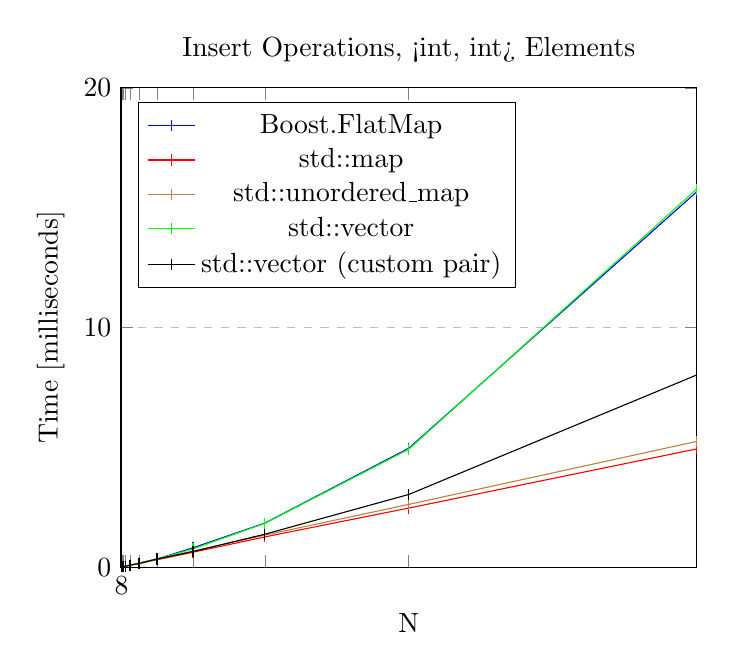
\begin{tikzpicture}
    \begin{axis}[
        width=3.5in,
        title={Insert Operations, <int, int> Elements},
        xlabel={N},
        ylabel={Time [milliseconds]},
        xmin=0, xmax=8192,
        ymin=0, ymax=20.0,
        xtick={8,16,32,64,128,256,512,1024,2048,4096,8192,16384},
        xticklabels={8,,,,,,,,,,,},
        ytick={0.0,10.0,20.0,30.0},
        legend pos=north west,
        ymajorgrids=true,
        grid style=dashed,
        scaled x ticks=false,
        scaled y ticks=true,
        legend entries={Boost.FlatMap,std::map,std::unordered\_map,std::vector,std::vector (custom pair)},
        ]

    \addplot[color=blue,mark=|,]
        coordinates {(8,0.0070956)(16,0.0112306)(32,0.0215942)(64,0.0414716)(128,0.0772576)(256,0.161137)(512,0.339035)(1024,0.803798)(2048,1.83769)(4096,4.9597)(8192,15.6539)};

    \addplot[color=red,mark=|,]
        coordinates {(8,0.0059762)(16,0.0107278)(32,0.0205472)(64,0.0423518)(128,0.0756524)(256,0.153538)(512,0.306883)(1024,0.62131)(2048,1.25993)(4096,2.46352)(8192,4.93078)};

    \addplot[color=brown,mark=|,]
        coordinates {(8,0.0076544)(16,0.0134522)(32,0.026009)(64,0.0420722)(128,0.0817146)(256,0.168821)(512,0.342698)(1024,0.664666)(2048,1.33619)(4096,2.61665)(8192,5.24265)};

    \addplot[color=green,mark=|,]
        coordinates {(8,0.005964)(16,0.0105752)(32,0.022433)(64,0.03763)(128,0.0762266)(256,0.156878)(512,0.33684)(1024,0.758057)(2048,1.82541)(4096,4.91914)(8192,15.7705)};

    \addplot[color=black,mark=|,]
        coordinates {(8,0.0058376)(16,0.0106448)(32,0.020044)(64,0.037086)(128,0.0832922)(256,0.149752)(512,0.337135)(1024,0.649203)(2048,1.37368)(4096,3.03122)(8192,8.01488)};

    \end{axis}
\end{tikzpicture}
\end{center}

\begin{center}
    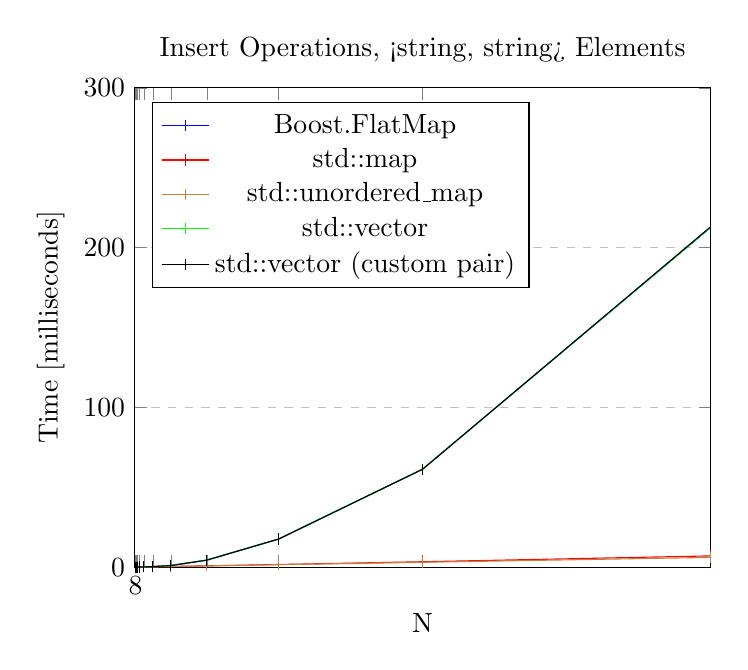
\begin{tikzpicture}
    \begin{axis}[
        width=3.5in,
        title={Insert Operations, <string, string> Elements},
        xlabel={N},
        ylabel={Time [milliseconds]},
        xmin=0, xmax=8192,
        ymin=0, ymax=300.0,
        xtick={8,16,32,64,128,256,512,1024,2048,4096,8192,16384},
        xticklabels={8,,,,,,,,,,,},
        ytick={0.0,100.0,200.0,300.0,400.0},
        legend pos=north west,
        ymajorgrids=true,
        grid style=dashed,
        scaled x ticks=false,
        scaled y ticks=true,
        legend entries={Boost.FlatMap,std::map,std::unordered\_map,std::vector,std::vector (custom pair)},
        ]

    \addplot[color=blue,mark=|,]
        coordinates {(8,0.0056294)(16,0.0113688)(32,0.0245568)(64,0.0521004)(128,0.123533)(256,0.331082)(512,0.973763)(1024,4.35386)(2048,17.5335)(4096,61.2927)(8192,212.469)};

    \addplot[color=red,mark=|,]
        coordinates {(8,0.0054754)(16,0.0101122)(32,0.02081)(64,0.0432052)(128,0.0850892)(256,0.179159)(512,0.377197)(1024,0.779511)(2048,1.62137)(4096,3.35122)(8192,7.00169)};

    \addplot[color=brown,mark=|,]
        coordinates {(8,0.0057274)(16,0.0112308)(32,0.0228528)(64,0.0448092)(128,0.0919372)(256,0.183631)(512,0.36901)(1024,0.740638)(2048,1.49183)(4096,2.9981)(8192,6.05877)};

    \addplot[color=green,mark=|,]
        coordinates {(8,0.0053228)(16,0.0113996)(32,0.024543)(64,0.0528586)(128,0.125005)(256,0.324659)(512,0.965707)(1024,4.37955)(2048,17.632)(4096,61.3544)(8192,212.515)};

    \addplot[color=black,mark=|,]
        coordinates {(8,0.0052376)(16,0.010924)(32,0.023371)(64,0.050662)(128,0.122445)(256,0.322264)(512,0.959212)(1024,4.35955)(2048,17.5875)(4096,61.2511)(8192,212.888)};

    \end{axis}
\end{tikzpicture}
\end{center}


As one might expect, insertionion takes longer in contiguous-storage
implementations.  Boost.FlatMap and a sorted \code{vector<pair<int, int>>}
have superlinear growth in insertion time.  While the curve for sorted
\code{vector} using a custom \code{struct} instead of a \code{pair} is
superlinear as well, it is dramatically flatter in its growth -- much closer
to node-based \code{map}.

\begin{center}
    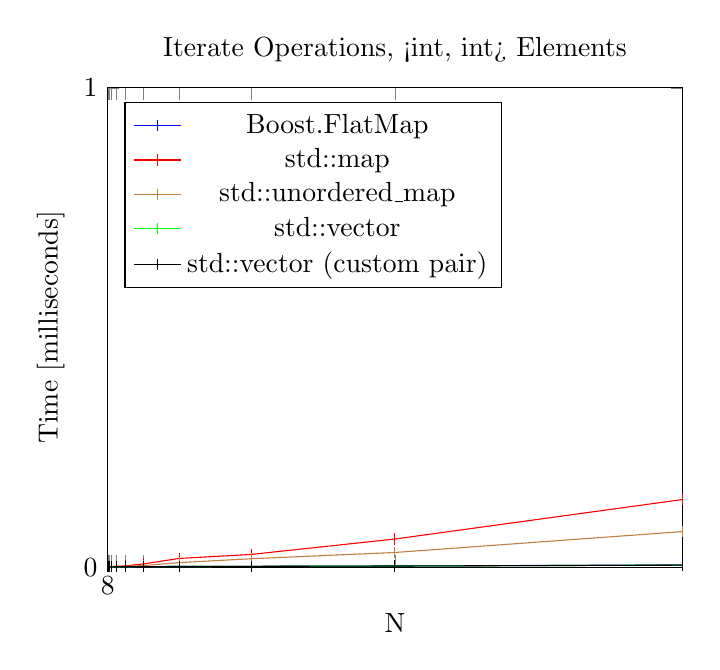
\begin{tikzpicture}
    \begin{axis}[
        width=3.5in,
        title={Iterate Operations, <int, int> Elements},
        xlabel={N},
        ylabel={Time [milliseconds]},
        xmin=0, xmax=8192,
        ymin=0, ymax=1.0,
        xtick={8,16,32,64,128,256,512,1024,2048,4096,8192,16384},
        xticklabels={8,,,,,,,,,,,},
        ytick={0.0,1.0,2.0},
        legend pos=north west,
        ymajorgrids=true,
        grid style=dashed,
        scaled x ticks=false,
        scaled y ticks=true,
        legend entries={Boost.FlatMap,std::map,std::unordered\_map,std::vector,std::vector (custom pair)},
        ]

    \addplot[color=blue,mark=|,]
        coordinates {(8,0.0005866)(16,0.0006144)(32,0.0006284)(64,0.0006982)(128,0.0006424)(256,0.0007542)(512,0.0009082)(1024,0.001299)(2048,0.0015082)(4096,0.002263)(8192,0.0044698)};

    \addplot[color=red,mark=|,]
        coordinates {(8,0.0007122)(16,0.0007126)(32,0.0010196)(64,0.0016064)(128,0.0015926)(256,0.0025004)(512,0.0065788)(1024,0.0180472)(2048,0.0264)(4096,0.0586108)(8192,0.141065)};

    \addplot[color=brown,mark=|,]
        coordinates {(8,0.0006146)(16,0.0006844)(32,0.0007404)(64,0.0009218)(128,0.0010058)(256,0.001648)(512,0.0031572)(1024,0.0093728)(2048,0.0174326)(4096,0.0305204)(8192,0.0741294)};

    \addplot[color=green,mark=|,]
        coordinates {(8,0.0005868)(16,0.0006288)(32,0.0006282)(64,0.000614)(128,0.0007544)(256,0.0007542)(512,0.000908)(1024,0.0012432)(2048,0.0015084)(4096,0.002277)(8192,0.0041346)};

    \addplot[color=black,mark=|,]
        coordinates {(8,0.0005866)(16,0.0006148)(32,0.0006426)(64,0.0005862)(128,0.0006566)(256,0.0007404)(512,0.0009356)(1024,0.0012436)(2048,0.0016066)(4096,0.0022906)(8192,0.0040368)};

    \end{axis}
\end{tikzpicture}
\end{center}

\begin{center}
    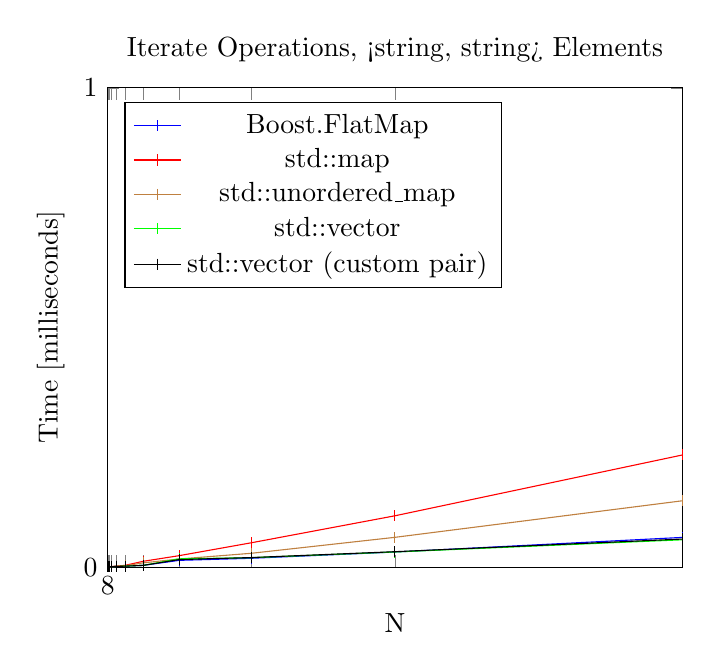
\begin{tikzpicture}
    \begin{axis}[
        width=3.5in,
        title={Iterate Operations, <string, string> Elements},
        xlabel={N},
        ylabel={Time [milliseconds]},
        xmin=0, xmax=8192,
        ymin=0, ymax=1.0,
        xtick={8,16,32,64,128,256,512,1024,2048,4096,8192,16384},
        xticklabels={8,,,,,,,,,,,},
        ytick={0.0,1.0,2.0},
        legend pos=north west,
        ymajorgrids=true,
        grid style=dashed,
        scaled x ticks=false,
        scaled y ticks=true,
        legend entries={Boost.FlatMap,std::map,std::unordered\_map,std::vector,std::vector (custom pair)},
        ]

    \addplot[color=blue,mark=|,]
        coordinates {(8,0.0006006)(16,0.0007128)(32,0.0007962)(64,0.0009498)(128,0.001285)(256,0.0020674)(512,0.0035338)(1024,0.0140938)(2048,0.0183962)(4096,0.0314566)(8192,0.0620052)};

    \addplot[color=red,mark=|,]
        coordinates {(8,0.0006006)(16,0.0007122)(32,0.00088)(64,0.0011876)(128,0.001872)(256,0.0036738)(512,0.0120966)(1024,0.023844)(2048,0.050649)(4096,0.107067)(8192,0.234094)};

    \addplot[color=brown,mark=|,]
        coordinates {(8,0.000698)(16,0.0007404)(32,0.0008382)(64,0.0010198)(128,0.0015228)(256,0.0027378)(512,0.0088278)(1024,0.016902)(2048,0.0287886)(4096,0.062117)(8192,0.138467)};

    \addplot[color=green,mark=|,]
        coordinates {(8,0.000587)(16,0.0007398)(32,0.0008938)(64,0.000908)(128,0.0012992)(256,0.0020394)(512,0.0036038)(1024,0.0172508)(2048,0.0195836)(4096,0.0315124)(8192,0.0570182)};

    \addplot[color=black,mark=|,]
        coordinates {(8,0.0006146)(16,0.0007262)(32,0.0008664)(64,0.00095)(128,0.0013828)(256,0.0020252)(512,0.003576)(1024,0.0156728)(2048,0.0199046)(4096,0.032127)(8192,0.0585828)};

    \end{axis}
\end{tikzpicture}
\end{center}


For all variants but \code{map}, iteration is relatively similar, and much
faster that \code{map}'s.

\begin{center}
    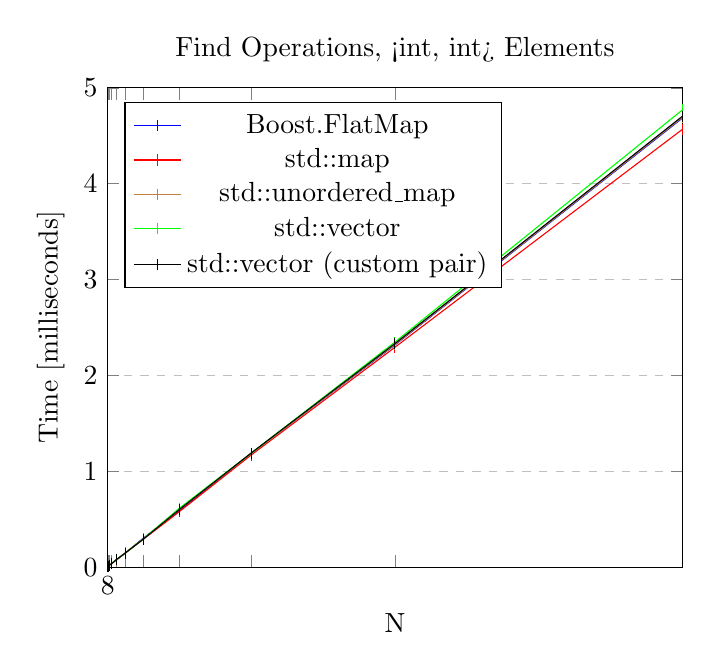
\begin{tikzpicture}
    \begin{axis}[
        width=3.5in,
        title={Find Operations, <int, int> Elements},
        xlabel={N},
        ylabel={Time [milliseconds]},
        xmin=0, xmax=8192,
        ymin=0, ymax=5.0,
        xtick={8,16,32,64,128,256,512,1024,2048,4096,8192,16384},
        xticklabels={8,,,,,,,,,,,},
        ytick={0.0,1.0,2.0,3.0,4.0,5.0,6.0},
        legend pos=north west,
        ymajorgrids=true,
        grid style=dashed,
        scaled x ticks=false,
        scaled y ticks=true,
        legend entries={Boost.FlatMap,std::map,std::unordered\_map,std::vector,std::vector (custom pair)},
        ]

    \addplot[color=blue,mark=|,]
        coordinates {(8,0.005015)(16,0.0101134)(32,0.019206)(64,0.0393078)(128,0.073684)(256,0.145284)(512,0.300651)(1024,0.583593)(2048,1.18364)(4096,2.31805)(8192,4.68716)};

    \addplot[color=red,mark=|,]
        coordinates {(8,0.0050146)(16,0.0096802)(32,0.019499)(64,0.0359672)(128,0.0723568)(256,0.145074)(512,0.288685)(1024,0.576876)(2048,1.16847)(4096,2.29383)(8192,4.56962)};

    \addplot[color=brown,mark=|,]
        coordinates {(8,0.0055462)(16,0.0104752)(32,0.0198508)(64,0.0366532)(128,0.0727744)(256,0.148873)(512,0.294408)(1024,0.596527)(2048,1.18301)(4096,2.32249)(8192,4.69465)};

    \addplot[color=green,mark=|,]
        coordinates {(8,0.0051964)(16,0.0102382)(32,0.0196804)(64,0.0383842)(128,0.0768818)(256,0.145088)(512,0.293207)(1024,0.612197)(2048,1.18783)(4096,2.34807)(8192,4.7723)};

    \addplot[color=black,mark=|,]
        coordinates {(8,0.0050988)(16,0.0105042)(32,0.0196114)(64,0.0363308)(128,0.0762108)(256,0.146234)(512,0.290498)(1024,0.598737)(2048,1.18911)(4096,2.33188)(8192,4.70609)};

    \end{axis}
\end{tikzpicture}
\end{center}

\begin{center}
    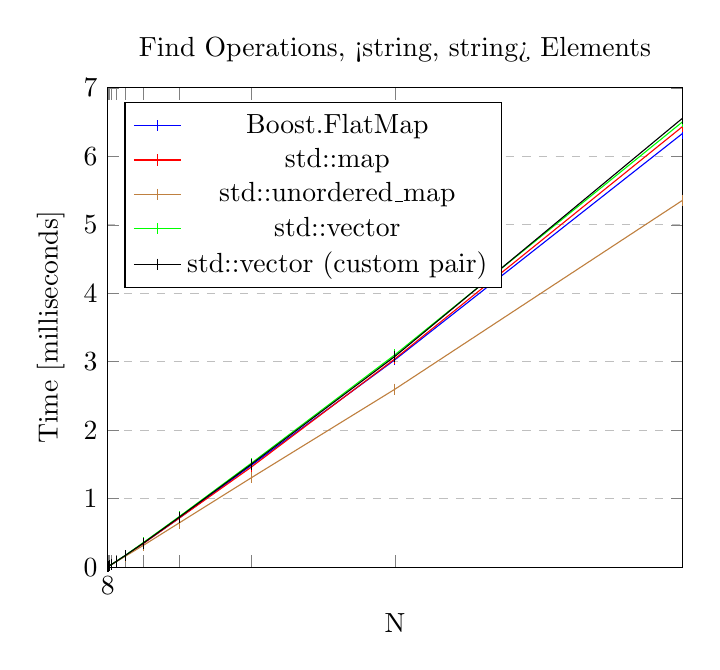
\begin{tikzpicture}
    \begin{axis}[
        width=3.5in,
        title={Find Operations, <string, string> Elements},
        xlabel={N},
        ylabel={Time [milliseconds]},
        xmin=0, xmax=8192,
        ymin=0, ymax=7.0,
        xtick={8,16,32,64,128,256,512,1024,2048,4096,8192,16384},
        xticklabels={8,,,,,,,,,,,},
        ytick={0.0,1.0,2.0,3.0,4.0,5.0,6.0,7.0,8.0},
        legend pos=north west,
        ymajorgrids=true,
        grid style=dashed,
        scaled x ticks=false,
        scaled y ticks=true,
        legend entries={Boost.FlatMap,std::map,std::unordered\_map,std::vector,std::vector (custom pair)},
        ]

    \addplot[color=blue,mark=|,]
        coordinates {(8,0.0049728)(16,0.0097228)(32,0.0196406)(64,0.0392518)(128,0.0800918)(256,0.168374)(512,0.344426)(1024,0.714195)(2048,1.48361)(4096,3.02826)(8192,6.3356)};

    \addplot[color=red,mark=|,]
        coordinates {(8,0.0047214)(16,0.0094566)(32,0.0192898)(64,0.0387618)(128,0.0803028)(256,0.165253)(512,0.342924)(1024,0.713987)(2048,1.45804)(4096,3.04201)(8192,6.43682)};

    \addplot[color=brown,mark=|,]
        coordinates {(8,0.005085)(16,0.0097218)(32,0.0195412)(64,0.038635)(128,0.077691)(256,0.156778)(512,0.315699)(1024,0.644474)(2048,1.3024)(4096,2.59859)(8192,5.35875)};

    \addplot[color=green,mark=|,]
        coordinates {(8,0.0049858)(16,0.0099452)(32,0.0199886)(64,0.0404808)(128,0.0830958)(256,0.169896)(512,0.356055)(1024,0.736257)(2048,1.51503)(4096,3.10195)(8192,6.5057)};

    \addplot[color=black,mark=|,]
        coordinates {(8,0.0051408)(16,0.0097912)(32,0.019961)(64,0.0400624)(128,0.0818706)(256,0.168359)(512,0.348797)(1024,0.727554)(2048,1.50018)(4096,3.07821)(8192,6.55891)};

    \end{axis}
\end{tikzpicture}
\end{center}


\code{find()} performance is roughly similar across all the
implementations, and they all show superlinear growth.  Note that
Boost.FlatMap performs the best here.

\begin{center}
    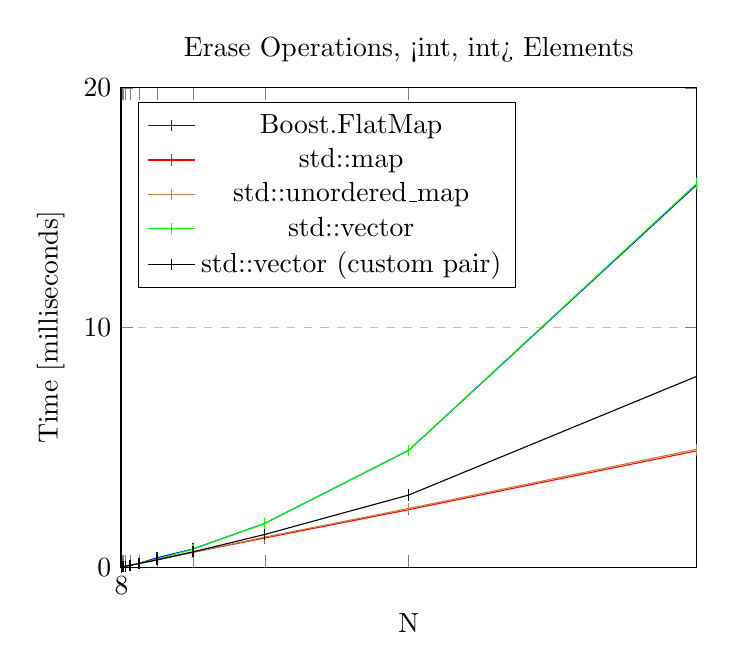
\begin{tikzpicture}
    \begin{axis}[
        width=3.5in,
        title={Erase Operations, <int, int> Elements},
        xlabel={N},
        ylabel={Time [milliseconds]},
        xmin=0, xmax=8192,
        ymin=0, ymax=20.0,
        xtick={8,16,32,64,128,256,512,1024,2048,4096,8192,16384},
        xticklabels={8,,,,,,,,,,,},
        ytick={0.0,10.0,20.0,30.0},
        legend pos=north west,
        ymajorgrids=true,
        grid style=dashed,
        scaled x ticks=false,
        scaled y ticks=true,
        legend entries={Boost.FlatMap,std::map,std::unordered\_map,std::vector,std::vector (custom pair)},
        ]

    \addplot[color=blue,mark=|,]
        coordinates {(8,0.0051968)(16,0.010001)(32,0.0199196)(64,0.0393356)(128,0.0753736)(256,0.158077)(512,0.387073)(1024,0.756719)(2048,1.82652)(4096,4.87614)(8192,15.9514)};

    \addplot[color=red,mark=|,]
        coordinates {(8,0.0054768)(16,0.0104486)(32,0.0201698)(64,0.0370032)(128,0.0751624)(256,0.148191)(512,0.299952)(1024,0.621442)(2048,1.21551)(4096,2.39683)(8192,4.84934)};

    \addplot[color=brown,mark=|,]
        coordinates {(8,0.0059918)(16,0.0112874)(32,0.0215106)(64,0.0385676)(128,0.0774258)(256,0.155735)(512,0.307876)(1024,0.616936)(2048,1.25192)(4096,2.4474)(8192,4.91601)};

    \addplot[color=green,mark=|,]
        coordinates {(8,0.005071)(16,0.0101262)(32,0.0197662)(64,0.0370584)(128,0.0801502)(256,0.156891)(512,0.329571)(1024,0.747009)(2048,1.82659)(4096,4.88021)(8192,16.0027)};

    \addplot[color=black,mark=|,]
        coordinates {(8,0.0052384)(16,0.009931)(32,0.0195128)(64,0.0364296)(128,0.0779854)(256,0.14865)(512,0.304689)(1024,0.634243)(2048,1.36407)(4096,3.00877)(8192,7.9576)};

    \end{axis}
\end{tikzpicture}
\end{center}

\begin{center}
    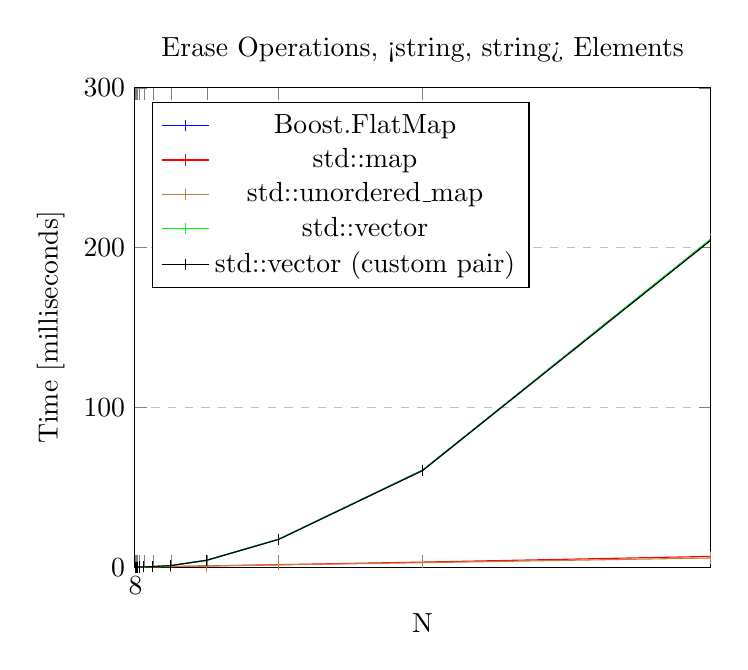
\begin{tikzpicture}
    \begin{axis}[
        width=3.5in,
        title={Erase Operations, <string, string> Elements},
        xlabel={N},
        ylabel={Time [milliseconds]},
        xmin=0, xmax=8192,
        ymin=0, ymax=300.0,
        xtick={8,16,32,64,128,256,512,1024,2048,4096,8192,16384},
        xticklabels={8,,,,,,,,,,,},
        ytick={0.0,100.0,200.0,300.0,400.0},
        legend pos=north west,
        ymajorgrids=true,
        grid style=dashed,
        scaled x ticks=false,
        scaled y ticks=true,
        legend entries={Boost.FlatMap,std::map,std::unordered\_map,std::vector,std::vector (custom pair)},
        ]

    \addplot[color=blue,mark=|,]
        coordinates {(8,0.0054618)(16,0.0105594)(32,0.0225284)(64,0.0507192)(128,0.120754)(256,0.323253)(512,0.956769)(1024,4.30449)(2048,17.4728)(4096,60.7224)(8192,205.014)};

    \addplot[color=red,mark=|,]
        coordinates {(8,0.0050712)(16,0.0099872)(32,0.019821)(64,0.0395304)(128,0.0812978)(256,0.173619)(512,0.358389)(1024,0.734809)(2048,1.52141)(4096,3.13507)(8192,6.69623)};

    \addplot[color=brown,mark=|,]
        coordinates {(8,0.005545)(16,0.0105354)(32,0.0210386)(64,0.0419678)(128,0.0835702)(256,0.168333)(512,0.33959)(1024,0.676251)(2048,1.37131)(4096,2.75454)(8192,5.69665)};

    \addplot[color=green,mark=|,]
        coordinates {(8,0.0052226)(16,0.0105444)(32,0.0223738)(64,0.0506704)(128,0.120826)(256,0.321113)(512,0.940469)(1024,4.18407)(2048,17.4925)(4096,60.5359)(8192,205.073)};

    \addplot[color=black,mark=|,]
        coordinates {(8,0.0053226)(16,0.0107308)(32,0.022096)(64,0.04977)(128,0.118991)(256,0.317389)(512,0.940927)(1024,4.28014)(2048,17.3208)(4096,60.4091)(8192,204.371)};

    \end{axis}
\end{tikzpicture}
\end{center}


Erasure has a similar performance profile to insertion, except that the sorted
\code{vector<pair<int, int>>} performs substantially better than
Boost.FlatMap.\\


\subsection{Implications}

TODO Iteration is vastly cheaper for contiguous-storage variants.  It has been
suggested that a \code{map} with a custom allocator can achieve similar
performance to flat data structures, but this would not apply to iteration
performance, unless the values were added to the \code{map} in sorted order.\\

In all the graphs above, the reason the custom-\code{pair} sorted vector
performs so much better than \code{vector<pair<int, int>>} seems to be that
the custom-\code{pair} type has \code{nothrow} special functions.
Implementing all the special functions and adding \code{nothrow(false)} to
each makes the custom-\code{pair} version perform identically to the
\code{pair<int, int>} version.

Boost.FlatMap differs quite a bit from a sorted \code{vector}.  Clearly there
are a lot of QOI choices to make in implementing a standard \code{flat_map}.
